\documentclass[12pt]{article}

\usepackage[utf8]{inputenc}
\usepackage[T1]{fontenc}
\usepackage[romanian]{babel}
\usepackage{amsmath}
\usepackage{amssymb}
\usepackage{array}
\usepackage{geometry}
\usepackage{xcolor}
\usepackage{graphicx}

\geometry{a4paper, margin=2.2cm}
\setlength{\parindent}{0pt}
\setlength{\parskip}{0.65em}

\title{
\textbf{Model matematic pentru engine-ul MiniScript+}\\
\large ScripticX - Learning Platform
}

\author{
\begin{tabular}{c}
realizat de Andrei Lascu \\
\small Colegiul Național ``Gheorghe Munteanu Murgoci'', Brăila \\[0.5em]
\small coordonator: Prof. Paul Pruș \\
\small Colegiul Național ``Gheorghe Munteanu Murgoci'', Brăila
\end{tabular}
}

\date{\small Mai 2026}

\begin{document}

\begin{titlepage}
\centering
\vspace*{2.5cm}

{\Large \textbf{ScripticX - Learning Platform}\par}
\vspace{1.2cm}

{\Huge \textbf{Model matematic}\par}
\vspace{0.25cm}
{\Huge \textbf{pentru engine-ul MiniScript+}\par}

\vspace{1.5cm}
{\large Document tehnic privind reprezentarea formală, execuția și analiza complexității limbajului MiniScript+\par}

\vfill

\begin{tabular}{c}
\textbf{Realizat de:} \\
Andrei Lascu \\
\small Colegiul Național ``Gheorghe Munteanu Murgoci'', Brăila \\[1.2em]
\textbf{Profesor coordonator:} \\
Prof. Paul Pruș \\
\small Colegiul Național ``Gheorghe Munteanu Murgoci'', Brăila
\end{tabular}

\vfill

{\large Mai 2026\par}

\end{titlepage}

\pagenumbering{roman}
\tableofcontents
\newpage
\pagenumbering{arabic}

\section{Introducere}

MiniScript+ este un limbaj educațional proiectat pentru a simplifica procesul de învățare a programării. Din punct de vedere matematic, un program MiniScript+ poate fi privit ca o structură formală alcătuită din instrucțiuni, expresii și un state intern care se modifică în timpul execuției programului.

Engine-ul MiniScript+ funcționează precum un interpretor, așadar primește codul sursă, îl transformă într-o reprezentare internă, apoi execută instrucțiunile pas cu pas. Fluxul principal poate fi observat mai jos:

\[
\text{Cod sursă}
\longrightarrow
\text{Tokenizare}
\longrightarrow
\text{Parsare}
\longrightarrow
\text{AST}
\longrightarrow
\text{Evaluare}
\longrightarrow
\text{Output}
\]

Această structură este facilă platformei deoarece ne permite atât rularea programului, cât și vizualizarea execuției programului, debugging-ul și estimarea complexității algoritmului.

\section{Modelul formal al programului}

Un program MiniScript+ poate fi reprezentat ca o secvență finită de instrucțiuni:

\[
P = (I_1, I_2, \ldots, I_n)
\]

unde fiecare instrucțiune \(I_i\) aparține unei mulțimi de instrucțiuni admise:

\[
I_i \in \mathcal{I}
\]
\\
\\
\\
Mulțimea instrucțiunilor poate fi descrisă astfel:

\[
\mathcal{I} =
\{
\text{INPUT},
\text{PRINT},
\text{ASSIGN},
\text{IF},
\text{ELSE},
\text{WHILE},
\text{END}
\}
\]

Astfel, un program nu este tratat doar ca text, ci ca o listă ordonată de operații care pot modifica state-ul intern al interpretorului.

\section{State-ul intern al interpretorului}

Deoarece în timpul execuției programului interpretorul nostru trebuie să rețină mai multe lucruri, precum variabilele, ce s-a afișat, linia curentă, câți pași au fost executați și ce input-uri mai sunt de citit, interpretorul păstrează un state intern. Acesta poate fi reprezentat printr-un tuplu:

\[
\sigma = (V, O, l, s, Q)
\]

unde:

\[
\begin{aligned}
V &= \text{tabelul variabilelor definite în program} \\
O &= \text{lista valorilor afișate la output} \\
l &= \text{linia curentă executată} \\
s &= \text{numărul de pași executați} \\
Q &= \text{coada valorilor de input}
\end{aligned}
\]

Tabelul variabilelor poate fi privit ca o funcție parțială:

\[
V : \text{Identificator} \rightarrow \text{Valoare}
\]

De exemplu, dacă în program apare instrucțiunea:

\[
X = 5
\]

atunci starea variabilelor se modifică astfel:

\[
V'(X) = 5
\]

iar pentru orice altă variabilă \(Y \neq X\):

\[
V'(Y) = V(Y)
\]

Pe scurt, folosind această metodă, creăm un "snapshot" al runtime-ului curent. :)

\section{Funcția de tranziție}

Execuția programului poate fi descrisă printr-o funcție de tranziție:

\[
\delta(\sigma, I_i) = \sigma'
\]

Aceasta înseamnă că, pornind de la o stare curentă \(\sigma\) și executând instrucțiunea \(I_i\), interpretorul obține o stare nouă \(\sigma'\).

De exemplu, pentru o atribuire de forma:

\[
X = expr
\]

tranziția poate fi descrisă prin:

\[
\delta(\sigma, X = expr) =
(V[X \leftarrow eval(expr, V)], O, l+1, s+1, Q)
\]

unde \(eval(expr, V)\) este valoarea expresiei calculate folosind variabilele curente.

Așadar, pentru o instrucțiune de afișare:

\[
PRINT \ expr
\]

tranziția devine:

\[
\delta(\sigma, PRINT \ expr) =
(V, O \cup \{eval(expr, V)\}, l+1, s+1, Q)
\]

Prin urmare, instrucțiunile MiniScript+ pot fi analizate în mod riguros ca fiind transformări asupra unui state intern.

\section{Procesul de Tokenizare}

Definim \textbf{Procesul de Tokenizarea} ca fiind acea etapă în care codul sursă este parcurs caracter cu caracter și împărțit în unități lexicale numite \textbf{token-uri}, fiind cunoscut și sub numele de \textbf{Lexer}.

Fie următoarea notație a codului sursă printr-un șir de caractere:

\[
C = c_1c_2 \ldots c_n
\]

atunci, \textbf{lexerul} construiește o secvență de token-uri astfel:

\[
L(C) = (t_1, t_2, \ldots, t_m)
\]

unde fiecare token \(t_i\) poate fi un identificator, un număr, un string, un operator, o paranteză sau un cuvânt cheie.

Să luăm următorul exemplu:

\[
\texttt{X = X + 1}
\]

în cazul acesta, secvența de cod devine:

\[
(\text{IDENT}(X), \text{OP}(=), \text{IDENT}(X), \text{OP}(+), \text{NUMBER}(1))
\]

Deoarece fiecare caracter este citit cel mult de un număr constant de ori, \textit{complexitatea procesului de tokenizare} este:

\[
T_{tokenizare}(n) = O(n)
\]

unde \(n\) este numărul de caractere din codul sursă.

\section{Procesul de parsare și construirea structurii programului}

Procesul de parsare verifică dacă token-urile respectă regulile limbajului și construiește reprezentarea (sau modelul) internă a programului.

La nivel simplificat, putem defini sau exprima gramatica limbajului astfel:

\[
\begin{aligned}
Program &\rightarrow Instr^* \\
Instr &\rightarrow Assign \mid Print \mid Input \mid If \mid While \\
Assign &\rightarrow id = Expr \\
Print &\rightarrow PRINT \ Expr \\
Input &\rightarrow INPUT \ id \\
If &\rightarrow IF \ Expr \ THEN \ Program \ (ELSE \ Program)? \ END \\
While &\rightarrow WHILE \ Expr \ Program \ END
\end{aligned}
\]

De asemenea, ținem cont de ordinea operațiilor (prioritatea operatorilor). Așadar, următoarea expresie:

\[
X + 2 \cdot Y
\]

trebuie interpretată astfel:

\[
X + (2 \cdot Y)
\]

Ordinea din exemplul de mai jos încalcă rigurozitatea regulilor de calcul la nivel de expresii:

\[
(X + 2) \cdot Y
\]

Parserul citește token-urile și construiește structuri pentru instrucțiuni, condiții, bucle și expresii. Presupunem că există \(m\) token-uri, iar fiecare token este procesat o singură dată sau de un număr constant de ori, atunci:

\[
T_{parsare}(m) = O(m)
\]

\section{Reprezentarea expresiilor prin AST}
Un arbore sintactic abstract, sau AST (\textit{Abstract Syntax Tree}), este o reprezentare ierarhică a structurii logice a codului. Spre deosebire de textul sursă, AST-ul elimină detaliile de scriere ale limbajului și păstrează doar relațiile esențiale dintre operatori, variabile, valori și instrucțiuni. Astfel, expresiile pot fi evaluate corect, respectând prioritatea operatorilor și ordinea de execuție.

Așadar, expresiile din MiniScript+ sunt reprezentate printr-un arbore sintactic abstract (AST):

\[
AST_{expr} = (N, E, r)
\]

unde:

\[
\begin{aligned}
N &= \text{mulțimea nodurilor arborelui} \\
E &= \text{mulțimea muchiilor părinte-copil} \\
r &= \text{rădăcina arborelui}
\end{aligned}
\]

Nodurile interne reprezintă operatori, iar frunzele reprezintă valori sau variabile. De exemplu, pentru expresia:

\[
\texttt{sum + i * 2}
\]

AST-ul poate fi reprezentat astfel:

\begin{center}
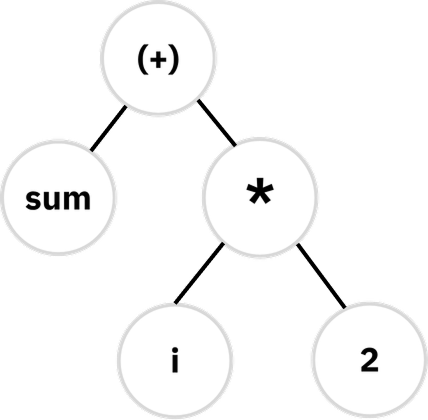
\includegraphics[width=0.40\textwidth]{expr_AST.png}
\end{center}

Această reprezentare este importantă deoarece păstrează ordinea corectă de evaluare și prioritatea operatorilor. În exemplul de mai sus, înmulțirea \(i \cdot 2\) este evaluată înaintea adunării cu variabila \texttt{sum}.

Același principiu se poate aplica și instrucțiunilor de control. De exemplu, o instrucțiune condițională de forma:

\[
\texttt{IF X > 10 THEN PRINT X}
\]

poate fi reprezentată printr-un arbore în care nodul principal este instrucțiunea \texttt{IF}, iar ramurile sale descriu condiția și blocul executat dacă expresia este adevărată:

\begin{center}
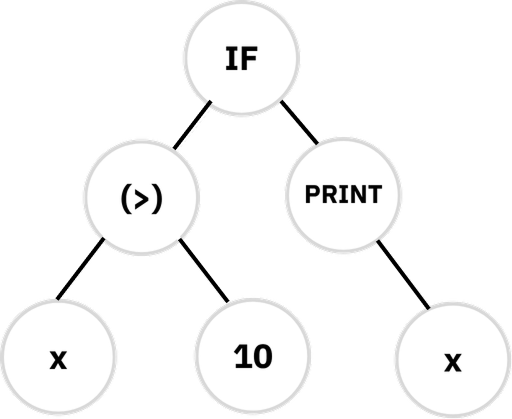
\includegraphics[width=0.55\textwidth]{if_AST.png}
\end{center}

În acest caz, nodul \texttt{IF} are \textbf{două componente principale}: expresia logică \(X > 10\) și instrucțiunea \texttt{PRINT X}. Astfel, folosind un AST putem descrie mai mult decât calcule aritmetice, extinzând reprezentarea până la structura logică a programului.

\section{Evaluarea recursivă a expresiilor}

În cadrul unui Arbore Sintactic Abstract, evaluarea unei expresii se realizează recursiv pe acesta. Definim următoarea funcție:

\[
eval : AST \times V \rightarrow \text{Valoare}
\]

Pentru o constantă numerică vom avea:

\[
eval(c, V) = c
\]

Pentru o variabilă, asemănător:

\[
eval(x, V) = V(x)
\]

Iar pentru o expresie binară:

\[
eval(a \ op \ b, V) =
eval(a, V) \ op \ eval(b, V)
\]

Să luăm următorul exemplu:

\[
eval(X + 2 \cdot Y, V)
=
V(X) + 2 \cdot V(Y)
\]

Dacă AST-ul unei expresii are \(k\) noduri, fiecare nod este vizitat o singură dată, deci:

\[
T_{evaluare\_expr}(k) = O(k)
\]

De asemenea, spațiul suplimentar folosit de evaluarea recursivă depinde în mod direct de înălțimea arborelui:

\[
S_{recursie} = O(h)
\]

unde \(h\) reprezintă înălțimea AST-ului.

\section{Despre execuția instrucțiunilor}

După parsare, programul este executat instrucțiune cu instrucțiune. Să presupunem că notăm prin \(p\) numărul de instrucțiuni efectiv executate, atunci:

\[
T_{executie} = O(p)
\]

\textbf{OBS:} Valoarea lui \(p\) nu este întotdeauna egală cu numărul de linii din program, deoarece buclele pot executa aceeași instrucțiune de mai multe ori.

Așadar, pentru o buclă cu verificare anterioară de tipul:

\[
WHILE \ cond \ DO \ B
\]

și blocul \(B\) are costul \(T_B\), iar condiția este adevărată de \(q\) ori, atunci costul total este aproximativ:

\[
T_{while} = O(q \cdot (T_{cond} + T_B))
\]

În schimb, pentru două bucle imbricate, cu \(q_1\) și \(q_2\) iterații:

\[
T_{nested} = O(q_1 \cdot q_2 \cdot T_B)
\]

Iar dacă ambele depind de aceeași dimensiune \(n\), obținem:

\[
T_{nested} = O(n^2)
\]

\section{Mecanismul de limitare al buclelor infinite}

Atunci când vorbim despre un limbaj de programare, un aspect important este modul în care acesta previne erorile din timpul runtime-ului, care pot fi și critice, în funcție de situație/context. Pentru siguranță, engine-ul MS+ folosește o limită maximă de pași:

\[
s \leq MAX\_STEPS
\]

La fiecare instrucțiune executată, contorul \(s\) crește:

\[
s' = s + 1
\]

Așadar, dacă condiția:

\[
s > MAX\_STEPS
\]

este adevărată, atunci execuția este oprită și programul este considerat potențial blocat într-o buclă infinită. Desigur, această măsură nu demonstrează matematic existența unei bucle infinite, dar previne blocarea aplicației în browser, limitând utilizatorul și avertizându-l atunci când o astfel de execuție este întâlnită.

\section{Complexitatea totală a engineului}

În final, procesarea completă a unui program MiniScript+, așa cum am văzut, include mai multe subprocese: tokenizare, parsare, construire AST și execuție:

\[
T_{total} =
T_{tokenizare} +
T_{parsare} +
T_{AST} +
T_{executie}
\]

Așadar, prin înlocuire:

\[
T_{total} = O(n) + O(m) + O(k) + O(p)
\]

deci:

\[
T_{total} = O(n + m + k + p)
\]

unde:

\[
\begin{aligned}
n &= \text{numărul de caractere din codul sursă} \\
m &= \text{numărul de token-uri generate} \\
k &= \text{numărul de noduri din AST} \\
p &= \text{numărul de instrucțiuni executate}
\end{aligned}
\]

\textbf{OBS}: Dacă toate aceste mărimi sunt raportate la dimensiunea totală a programului, notată cu \(N\), atunci pentru etapa de procesare statică:

\[
T_{static} = O(N)
\]

Execuția poate deveni mai mare decât \(O(N)\) dacă programul conține bucle care rulează de multe ori.

\section{Complexitatea în spațiu}

Spațiul folosit de engine-ul MS+ provine din mai multe structuri interne:

\[
S_{total} =
S_{tokens} +
S_{AST} +
S_{variabile} +
S_{recursie} +
S_{output}
\]

Așadar, prin aproximare obținem:

\[
S_{total} = O(m + k + v + h + o)
\]

unde:

\[
\begin{aligned}
m &= \text{numărul de token-uri} \\
k &= \text{numărul de noduri din AST} \\
v &= \text{numărul de variabile distincte} \\
h &= \text{înălțimea maximă a AST-ului} \\
o &= \text{numărul de valori afișate la output}
\end{aligned}
\]

De obicei, în cadrul programelor educaționale, output-ul și numărul de variabile sunt mici, iar spațiul este asimilat de token-uri și AST:

\[
S_{total} \approx O(m + k)
\]
Desigur, asta nu înseamnă că este un lucru fixat. Se pot realiza și programe complexe dpdv. al utilizării resurselor disponibile.

\section{Despre Analizatorul de Complexitate}

\textbf{Analizatorul de Complexitate} extinde capabilitatea engine-ului, evaluând prin aproximare complexitatea programului. Acesta nu execută programul pentru toate valorile posibile de input. În schimb, el estimează complexitatea pe baza structurii sintactice a codului. Sistemul identifică următoarele caracteristici:

\[
\begin{aligned}
L &= \text{numărul total de bucle} \\
d &= \text{adâncimea maximă a buclelor imbricate} \\
v &= \text{numărul de variabile folosite} \\
b &= \text{numărul de blocuri condiționale}
\end{aligned}
\]

O estimare simplificată pentru complexitatea în timp este:

\[
C_{time} \approx O(n^d)
\]

unde \(d\) este adâncimea maximă a buclelor imbricate detectate. Putem observa în tabelul de mai jos exemplificat:

\[
\begin{array}{|c|c|}
\hline
\textbf{Structura programului} & \textbf{Complexitate estimată} \\
\hline
\text{fără bucle relevante} & O(1) \\
\hline
\text{o buclă simplă} & O(n) \\
\hline
\text{două bucle imbricate} & O(n^2) \\
\hline
\text{trei bucle imbricate} & O(n^3) \\
\hline
\end{array}
\]

Atunci când vine vorba de complexitatea în spațiu, analizatorul urmărește variabilele și structurile auxiliare:

\[
C_{space} \approx O(v + a)
\]

unde \(a\) reprezintă eventuale structuri auxiliare detectate. În versiunea educațională a MiniScript+, unde accentul este pus pe variabile simple și control de flux, estimarea spațiului este de obicei:

\[
C_{space} = O(1)
\]

dacă nu există structuri care cresc odată cu input-ul. Desigur, asta nu înseamnă că acesta va fi mereu constant.

\section{Calcularea scorului de eficiență}

Pentru a oferi feedback vizual, analizatorul poate transforma informațiile structurale într-un scor de eficiență astfel:

\[
Score = 100 - \alpha L - \beta d - \gamma b
\]

unde:

\[
\begin{aligned}
L &= \text{numărul de bucle} \\
d &= \text{adâncimea maximă a buclelor} \\
b &= \text{numărul de blocuri condiționale} \\
\alpha,\beta,\gamma &= \text{coeficienți de penalizare}
\end{aligned}
\]

Acest scor nu reprezintă o demonstrație formală a performanței, ci o aproximare la nivel educațional care ajută utilizatorul să observe dacă soluția are multe bucle sau blocuri imbricate.

\section{Exemplu de analiză}

Să luăm concret următorul program:

\[
\begin{array}{l}
\texttt{X = 0} \\
\texttt{WHILE X < N} \\
\quad \texttt{PRINT X} \\
\quad \texttt{X = X + 1} \\
\texttt{END}
\end{array}
\]

există o singură buclă, deci:

\[
d = 1
\]

Dacă bucla rulează de \(N\) ori, complexitatea în timp este:

\[
T(N) = O(N)
\]

Numărul de variabile folosite este constant, deci:

\[
S(N) = O(1)
\]

Pentru două bucle imbricate:

\[
\begin{array}{l}
\texttt{I = 0} \\
\texttt{WHILE I < N} \\
\quad \texttt{J = 0} \\
\quad \texttt{WHILE J < N} \\
\quad \quad \texttt{PRINT I + J} \\
\quad \quad \texttt{J = J + 1} \\
\quad \texttt{END} \\
\quad \texttt{I = I + 1} \\
\texttt{END}
\end{array}
\]

adâncimea maximă este:

\[
d = 2
\]

iar complexitatea estimată este:

\[
T(N) = O(N^2)
\]

\section{Observații privind corectitudinea analizei}

De ținut cont este faptul că \textbf{Analizatorul de Complexitate} oferă o estimare \textbf{euristică}. Acesta folosește structura codului, nu o demonstrație matematică completă pentru orice input posibil. De exemplu, o buclă de forma:

\[
\texttt{WHILE X < 10}
\]

poate avea un număr constant de iterații, deci complexitatea ei poate fi tratată ca:

\[
O(1)
\]

în timp ce o buclă dependentă de input:

\[
\texttt{WHILE X < N}
\]

este estimată ca:

\[
O(n)
\]

Prin urmare, scopul analizatorului este educațional: să ofere începătorului o aproximare clară a eficienței algoritmului și să evidențieze impactul buclelor, al imbricării și al structurii codului.

\section{Concluzie}

Engine-ul MiniScript+ poate fi descris matematic ca un interpretor bazat pe transformări succesive ale codului: de la procesul de tokenizare, parsare, construire AST până la evaluare. Fiecare instrucțiune modifică un state intern, iar expresiile sunt evaluate recursiv pe baza arborelui sintactic abstract.

Desigur, această abordare permite implementarea și extinderea funcționalității limbajului de programare: rularea programelor, debugging pas cu pas, evidențierea liniei curente și estimarea complexității algoritmului. Astfel, \textbf{MiniScript+} nu este doar un \textbf{limbaj educațional simplificat}, ci și un model practic pentru înțelegerea modului în care funcționează un interpretor.

\end{document}
